\documentclass[9pt]{article}
\usepackage{amsfonts}
\usepackage{amssymb}
\usepackage{amsmath}
\usepackage{amsthm}
\usepackage{latexsym}
\usepackage{graphicx}
\usepackage{geometry}
\usepackage{hyperref}
\usepackage{color}

% for bold \mathcal font
\usepackage{bm}

\textwidth 15.5cm
\textheight 22.5cm
\oddsidemargin 0pt
\evensidemargin 0pt
\topmargin 0cm

\newcommand{\V}[1]{\boldsymbol{#1}}
\newcommand{\IN}{{\mathbb{N}}}
\newcommand{\IZ}{{\mathbb{Z}}}
\newcommand{\IR}{{\mathbb{R}}}
\newcommand{\IC}{{\mathbb{C}}}
\newcommand{\QED}{\fbox{}}
\newcommand{\btau}{\mbox{\boldmath $\tau$}}

\setlength{\marginparwidth}{0.75in}
\newcommand{\MarginPar}[1]{\marginpar{\vskip-\baselineskip\raggedright\tiny\sffamily\hrule\smallskip{\color{red}#1}\par\smallskip\hrule}}

% for non-stacked fractions
\newcommand{\sfrac}[2]{\mathchoice
  {\kern0em\raise.5ex\hbox{\the\scriptfont0 #1}\kern-.15em/
   \kern-.15em\lower.25ex\hbox{\the\scriptfont0 #2}}
  {\kern0em\raise.5ex\hbox{\the\scriptfont0 #1}\kern-.15em/
   \kern-.15em\lower.25ex\hbox{\the\scriptfont0 #2}}
  {\kern0em\raise.5ex\hbox{\the\scriptscriptfont0 #1}\kern-.2em/
   \kern-.15em\lower.25ex\hbox{\the\scriptscriptfont0 #2}}
  {#1\!/#2}}

\renewcommand{\topfraction}{0.9}
\renewcommand{\bottomfraction}{0.9}
\renewcommand{\textfraction}{0.2}

\def\Fb {{\bf F}}
\def\gb {{\bf g}}
\def\mb {{\bf m}}
\def\ub {{\bf u}}
\def\bA {\bm{\mathcal{A}}}
\def\bB {\bm{\mathcal{B}}}
\def\bI {\bm{\mathcal{I}}}
\def\bR {\bm{\mathcal{R}}}

\def\taub {\boldsymbol{\tau}}
\def\psib {\boldsymbol{\psi}}

\def\half   {\frac{1}{2}}
\def\myhalf {\sfrac{1}{2}}

% Set the beginning of a LaTeX document
\begin{document}

\title{Effective Preconditioners for Stokes Problems}

%\author{ Mingchao Cai \footnote{Department of
%Mathematics, }}

\date{}          % Enter your date or \today between curly braces
\maketitle

%\begin{abstract}
%Existing methods for solving time dependent/independent Stokes problems.
%\end{abstract}

%
%{\bf Keywords} Multi-modeling, Decoupled preconditioning, Fluid flow
%coupled with porous media flow, Navier-Stokes equations, Darcy's
%law, Saddle-point problem.


\section{Stokes Equations, Projection Method and Preconditioners.}
\subsection{Projection Method.}
The Stokes equations are as follows
\begin{equation}\label{Time_Stokes}
 \left \{
        \begin{array} {ll}
                \V{\rho}\frac{\partial{\bf u}}{\partial t} -\mu \Delta{\bf u}+\nabla p
                      =\mathbf{f}, \\
                 \nabla\cdot{\bf u}=-g.
        \end{array}
               \right.
\end{equation}
Here, ${\bf u}$ is the velocity, $p$ is the pressure, $\V{\rho}$ is the density function, $\mu$ is the viscosity, ${\bf f}$ is the external force and $g$ is the source term.


By using MAC discretization, together with a backward Euler method, we obtain a linear system of the following form,
\begin{equation}\label{Saddle_operator}
{\bf M} \left(\begin{array}{c}
{\bf u}^{(n+1)} \\
p^{(n+1)}
\end{array}\right)=
\left(\begin{array}{cc}
{\bf A} & {\bf G} \\
-{\bf D} & {\bf 0}
\end{array}\right)
\left(\begin{array}{c}
{\bf u}^{(n+1)} \\
p^{(n+1)}
\end{array}\right)=
\left(\begin{array}{c}
 {\bf f}^{(n)} \\
 g^{(n)}
\end{array}\right).
\end{equation}
Here, ${\bf A}=\frac{\V{\rho}}{\Delta t}{\bf I} - \mu {\bf L}$ (with ${\V{\rho}}$ being a diagonal matrix) is the discrete operator for $\frac{\V{\rho}}{\Delta t}{\bf I}-\mu  {\bf \Delta}$, ${\bf D}$ for $\nabla \cdot$, and ${\bf G}$ for $\nabla$, ${\bf f}^{(n)}$ includes both the force term at $t_n$ and the velocity at $t_n$ divided by $\Delta t$. Moreover, we have ${\bf D}=-{\bf G}^*$ and ${\bf D}{\bf G}={\bf L}_p$ is the discrete Laplacian operator. To differentiate the time dependent operator  with stationary operator, we will use ${\bf A}_0=-\mu  {\bf L}$ for $-\mu  {\bf \Delta}$ in the subsequent presentation.

The projection algorithm \cite{BellCollelaGlaz, Chorin} for the variable density Stokes equations is as follows.

Step 1: Using implicit viscosity step to solve for an intermediate velocity ${\bf u}^*$:
\begin{equation}\label{implicit_velocity}
\left( \frac{\V{\rho}}{\Delta t} {\bf I}+{\bf A}_0 \right){\bf u}^*= {\bf f}^{(n)}.
\end{equation}

Step 2: Solve the variable density pressure Poisson problem to get $\phi$.
\begin{equation}\label{pre_Poisson_eqn}
-\left({\bf D} \V{\rho}^{-1} {\bf G}\right) \phi =  -  \frac{1}{\Delta t}\left({\bf D} {\bf u}^*+g^{(n)}\right).
\end{equation}

Step 3: Update the velocity
$$
{\bf u}^{(n+1)}={\bf u}^* - \Delta t {\V{\rho}}^{-1} {\bf G} \phi.
$$

Step 4: Correct the pressure term by using
\begin{equation}\label{pressure_correction}
p^{(n+1)}=\phi -  \Delta t \mu  \left({\bf D} {\V{\rho}}^{-1} {\bf G} \right)\phi.
\end{equation}
In the 2nd and the 3rd step of the above projection algorithm, we project ${\bf u}^*$ into divergence free space, i.e.,
\begin{equation}\label{time_update}
\frac{{\bf u}^{(n+1)}-{\bf u}^*}{\Delta t}= -{\V{\rho}}^{-1} {\bf G} \phi,
\end{equation}
with ${\bf u}^{(n+1)}$ satisfying
$$
- {\bf D} {\bf u}^{(n+1)} = g^{(n)}.
$$
The 4th step of the above algorithm (pressure correction) is based on the following arguments.

Applying $\left( \frac{\V{\rho}}{\Delta t} {\bf I}+{\bf A}_0 \right)$ to both sides of (\ref{time_update}), noting that ${\bf u}^{(n+1)}$ and $p^{(n+1)}$ satisfy the discrete Stokes equation (\ref{Saddle_operator}) and ${\bf u}^*$ satisfies (\ref{implicit_velocity}), we derive that
\begin{equation}\label{pre_corr_der}
-{\bf G} p^{(n+1)} =- \Delta t \left( \frac{\V{\rho}}{\Delta t} {\bf I}+{\bf A}_0 \right)  {\V{\rho}}^{-1} {\bf G} \phi.
\end{equation}
multiplying both sides of (\ref{pre_corr_der}) by ${\bf D}$, we get
$$
{\bf L}_{p} p^{(n+1)}={\bf L}_{p} \phi + \Delta t {\bf D} {\bf A}_0 {\V{\rho}}^{-1} {\bf G} \phi.
$$
Therefore, the pressure correction should be
$$
p^{(n+1)}= \phi + \Delta t {\bf L}_{p}^{-1}{\bf D}{\bf A}_0 {\V{\rho}}^{-1} {\bf G} \phi.
$$

In \cite{Griffith}, by assuming
$$
{\bf L}_p^{-1} {\bf D} {\bf A}_0 \approx {\bf D},
$$
(which is true for constant viscosity and periodic boundaries), we obtain (\ref{pressure_correction}).

({\it Alternatively, multiplying both sides of (\ref{pre_corr_der}) by ${\bf D}{\V{\rho}}^{-1}$, we get
$$
{\bf L}_{\V{\rho}} p^{(n+1)}={\bf L}_{\V{\rho}} \phi + \Delta t {\bf D} {\V{\rho}}^{-1} ({\bf A}_0 {\V{\rho}}^{-1} {\bf G} \phi).
$$
Here, we define ${\bf L}_{\V{\rho}}={\bf D} \V{\rho}^{-1} {\bf G}$.
Therefore, the pressure correction should be
$$
p^{(n+1)}= \phi + \Delta t {\bf L}_{\V{\rho}}^{-1}{\bf D}{\V{\rho}}^{-1} ({\bf A}_0 {\V{\rho}}^{-1} {\bf G} \phi).
$$
})

\subsection{Robust Preconditioners.}
The Stokes system (\ref{Saddle_operator}) is solved by using GMRES method (since preconditioners are nonsymmetric) with various preconditioners. There are 3 preconditioners we are going to study and investigate.

{\bf Projection Preconditioner.} We denote the discrete variable density Laplacian operator as $L_{\V{\rho}}  = {\bf D} \V{\rho}^{-1} {\bf G}$. The above 4 steps of projection algorithm can be written into
\begin{equation}\label{P3_variable_density}
{\bf P}_3^{-1}=\left(\begin{array}{cc}
{\bf I} & - {\V{\rho}}^{-1}{\bf G} \\
{\bf 0}      & \frac{1}{\Delta t}{\bf I}- \mu {\bf L}_{\V{\rho}}
\end{array}\right)
\left(\begin{array}{cc}
{\bf I}     &  {\bf 0} \\
{\bf 0}     &  -{\bf L}_{\V{\rho}}^{-1}
\end{array}\right)
\left(\begin{array}{cc}
{\bf I}     &  {\bf 0} \\
-{\bf D}     &  -{\bf I}
\end{array}\right)
\left(\begin{array}{cc}
{\bf A}^{-1}       & {\bf 0} \\
{\bf 0}            & {\bf I}
\end{array}\right).
\end{equation}
If ${\V{\rho}}=const=\rho {\bf I}$, ${\bf P}_3^{-1}$ is equivalent to
\begin{equation}\label{Boyce_precon}
{\bf P}_3^{-1}=\left(\begin{array}{cc}
{\bf I}   & -\frac{\Delta t}{\rho} {\bf G} \\
{\bf 0}   & {\bf I}-\frac{\Delta t}{\rho}\mu {\bf L}_p
\end{array}\right)
\left(\begin{array}{cc}
{\bf I}     &  {\bf 0} \\
{\bf 0}     &  -{\bf L}_p^{-1}
\end{array}\right)
\left(\begin{array}{cc}
{\bf I}     &  {\bf 0} \\
-\frac{\rho}{\Delta t}{\bf D}     &  -\frac{\rho}{\Delta t}{\bf I}
\end{array}\right)
\left(\begin{array}{cc}
{\bf A}^{-1}       & {\bf 0} \\
{\bf 0}            & {\bf I}
\end{array}\right).
\end{equation}
or
\begin{equation}\label{Boyce_precon_equ}
{\bf P}_3^{-1}=\left(\begin{array}{cc}
{\bf I} & - {\bf G} \\
{\bf 0}      & \frac{\rho}{\Delta t}{\bf I}- \mu {\bf L}_p
\end{array}\right)
\left(\begin{array}{cc}
{\bf I}     &  {\bf 0} \\
{\bf 0}     &  -{\bf L}_p^{-1}
\end{array}\right)
\left(\begin{array}{cc}
{\bf I}     &  {\bf 0} \\
-{\bf D}     &  -{\bf I}
\end{array}\right)
\left(\begin{array}{cc}
{\bf A}^{-1}       & {\bf 0} \\
{\bf 0}            & {\bf I}
\end{array}\right).
\end{equation}
When $\rho=0$, (\ref{Boyce_precon_equ}) is reduced to the following steady state preconditioner (\ref{Boyce_pre_steady}).
\begin{equation}\label{Boyce_pre_steady}
\tilde{{\bf P}_3}^{-1}=\left(\begin{array}{cc}
{\bf I}      & -{\bf G} \\
{\bf 0}      & -\mu {\bf L}_p
\end{array}\right)
\left(\begin{array}{cc}
{\bf I}      & {\bf 0} \\
{\bf 0}      & -{\bf L}_p^{-1}
\end{array}\right)
\left(\begin{array}{cc}
{\bf I}      &  {\bf 0} \\
-{\bf D}     &  -{\bf I}
\end{array}\right)
\left(\begin{array}{cc}
{\bf A}_0^{-1}     & {\bf 0} \\
{\bf 0}            & {\bf I}
\end{array}\right).
\end{equation}
To link ${\bf P}_3$ with the original saddle point form (\ref{Saddle_operator}), we check (constant density case)
\begin{eqnarray}\label{preconditioned_sys}
{\bf P_3}^{-1} {\bf M} &=&
\left(\begin{array}{cc}
{\bf I} & - {\bf G} \\
{\bf 0}      & \frac{\rho}{\Delta t}{\bf I}- \mu {\bf L}_p
\end{array}\right)
\left(\begin{array}{cc}
{\bf I}     &  {\bf 0} \\
{\bf 0}     &  -{\bf L}_p^{-1}
\end{array}\right)
\left(\begin{array}{cc}
{\bf I}      &   {\bf 0} \\
-{\bf D}     &  -{\bf I}
\end{array}\right)
\left(\begin{array}{cc}
{\bf A}^{-1}       & {\bf 0} \\
{\bf 0}            & {\bf I}
\end{array}\right)
\left(\begin{array}{cc}
{\bf A}       & {\bf G} \\
-{\bf D}      & {\bf 0}
\end{array}\right) = \cr
&=& \left(\begin{array}{cc}
{\bf I}        & ({\bf I}-{\bf G}{\bf L}_p^{-1}{\bf D}){\bf A}^{-1} {\bf G} \\
{\bf 0}        & (\frac{\rho}{\Delta t} {\bf L}_p^{-1} -\mu {\bf I}) {\bf D} {\bf A}^{-1}{\bf G}
\end{array}\right).
\end{eqnarray}
Note that ${\bf A} = \frac{\rho}{\Delta t} {\bf I} - \mu {\bf L}$, when boundary condition is periodic, the basic operators ${\bf G}$, ${\bf D}$, ${\bf A}$ and ${\bf L}_p$ are commutative, ${\bf P}_3^{-1} {\bf M}$ is exactly the discrete identity operator.

{\bf A. Wathen's Preconditioner (same as R. Winther's Preconditioner)}. The block triangular preconditioner in the sense of \cite{MardalWinther2004, Griffith} for Stokes problem is
\begin{equation}\label{Wathen_Pre_variable_den}
{\bf P}_2^{-1}=\left(\begin{array}{cc}
{\bf A}^{-1} & {\bf 0} \\
{\bf 0}      & {\bf I}
\end{array}\right)
\left(\begin{array}{cc}
{\bf I}     & -{\bf G} \\
{\bf 0}     &  {\bf I}
\end{array}\right)
\left(\begin{array}{cc}
{\bf I}       & {\bf 0} \\
{\bf 0}       & \frac{1}{\Delta t} {\bf L}_{\V{\rho}}^{-1} - \mu {\bf I}
\end{array}\right).
\end{equation}
If ${\V{\rho}}=const=\rho {\bf I}$, then $-\frac{1}{\Delta t} {\bf L}_{\V{\rho}}^{-1}=-\frac{\rho}{\Delta t} {\bf L}_p^{-1}$, one can also write several equivalent forms of ${\bf P}_2^{-1}$ corresponding to (\ref{Boyce_precon}), (\ref{Boyce_precon_equ}) and (\ref{Boyce_pre_steady}). This preconditioner is a Shcur complement approximation based preconditioner. More clearly, the Schur complement
$$
-{\bf D} {\bf A}^{-1} {\bf G}  = -{\bf D} \left(\begin{array}{cc}
\frac{\rho}{\Delta t} {\bf I} - \mu {\bf L} & {\bf 0} \\
{\bf 0}      & \frac{\rho}{\Delta t} {\bf I} - \mu {\bf L}
\end{array}\right)^{-1} {\bf G}
\approx -{\bf D}{\bf G} \left(\frac{\rho}{\Delta t} {\bf I} - \mu  {\bf L}_p \right)^{-1} =  -{\bf L}_p \left(\frac{\rho}{\Delta t} {\bf I} - \mu {\bf L}_p \right)^{-1}
$$
Therefore, the inverse of the Schur complement is approximately equal to  $-\frac{\rho}{\Delta t} {\bf L}_p^{-1} + \mu {\bf I}$.
%When the density is non-constant, we see that (\ref{Wathen_Pre_variable_den}) corresponds to Schur complement approximation %based preconditioner.
%When ${\V\rho}={\bf 0}$, (\ref{Wathen_Pre_variable_den}) is reduced to the preconditioner for steady state problem:
%$$
%%\begin{equation}\label{Schur_pre_steady}
%{\tilde P_2}=\left(\begin{array}{cc}
%{\bf A}_0 & {\bf G} \\
%{\bf 0}         & {\mu }^{-1} {\bf I}
%\end{array}\right).
%%\end{equation}
%$$

{\bf Modified projection preconditioner.}

From the algorithm derivation in Section 1.1, the modified projection preconditioner is
\begin{equation}\label{P4_variable_density}
P_4^{-1}=\left(\begin{array}{cc}
{\bf I} & - {\V{\rho}}^{-1}{\bf G} \\
{\bf 0}      & \frac{1}{\Delta t}{\bf I}+{\bf L}_p^{-1} {\bf D} {\bf A}_0 {\V{\rho}}^{-1} {\bf G}
\end{array}\right)
\left(\begin{array}{cc}
{\bf I}     &  {\bf 0} \\
{\bf 0}     &  -{\bf L}_{\V{\rho}}^{-1}
\end{array}\right)
\left(\begin{array}{cc}
{\bf I}      &  {\bf 0} \\
-{\bf D}     &  -{\bf I}
\end{array}\right)
\left(\begin{array}{cc}
{\bf A}^{-1}       & {\bf 0} \\
{\bf 0}            & {\bf I}
\end{array}\right).
\end{equation}
If ${\V{\rho}}=const=\rho {\bf I}$,  $\frac{1}{\Delta t} -{\bf L}_{\V{\rho}}^{-1}=-\frac{\rho}{\Delta t} {\bf L}_p^{-1}$, ${\bf P}_4^{-1}$ is equivalent to
\begin{equation}\label{Modified_Proj_Pre}
{\bf P}_4^{-1}=\left(\begin{array}{cc}
{\bf I} & -{\Delta t} {\V{\rho}}^{-1} {\bf G} \\
{\bf 0}      & {\bf I}+{\Delta t} {\V{\rho}}^{-1} {\bf L}_p^{-1} {\bf D} {\bf A}_0 {\bf G}
\end{array}\right)
\left(\begin{array}{cc}
{\bf I}     &  {\bf 0} \\
{\bf 0}     &  -{\bf L}_p^{-1}
\end{array}\right)
\left(\begin{array}{cc}
{\bf I}     &  {\bf 0} \\
-\frac{\V{\rho}}{\Delta t}{\bf D}     &  -\frac{\V{\rho}}{\Delta t}{\bf I}
\end{array}\right)
\left(\begin{array}{cc}
{\bf A}^{-1}       & {\bf 0} \\
{\bf 0}            & {\bf I}
\end{array}\right),
\end{equation}
if ${\V {\rho}}=const=\rho {\bf I}$, (\ref{modified_precon_equ}) is equivalent to
\begin{equation}\label{modified_precon_equ}
{\bf P}_4^{-1}=\left(\begin{array}{cc}
{\bf I} & - {\bf G} \\
{\bf 0}      & \frac{\rho}{\Delta t}{\bf I}+{\bf L}_p^{-1} {\bf D} {\bf A}_0 {\bf G}
\end{array}\right)
\left(\begin{array}{cc}
{\bf I}     &  {\bf 0} \\
{\bf 0}     &  -{\bf L}_p^{-1}
\end{array}\right)
\left(\begin{array}{cc}
{\bf I}     &  {\bf 0} \\
-{\bf D}     &  -{\bf I}
\end{array}\right)
\left(\begin{array}{cc}
{\bf A}^{-1}       & {\bf 0} \\
{\bf 0}            & {\bf I}
\end{array}\right).
\end{equation}
When the boundary condition is periodic, $P_4$ is reduced to $P_3$.
%{\bf Remark} For the modified projection preconditioner $P_4$ here, $\V{\rho}^{-1}$ should be scaled in front of ${\bf G}$.

For the projection preconditioner ${\bf P}_3$ and ${\bf P}_4$, one can justify its advantages from different points of view (the performance \cite{Griffith} and various interpretations of projection method). For periodic boundary condition, one can show that the preconditioned system converges in 1 iteration by using algebraic calculation or Fourier analysis. For ${\bf P}_2$, one can prove that only 2 iterations will be need for periodic boundaries. For non-periodic boundary condition, we can also prove that the eigenvalues of preconditioned system ${\bf P}_2^{-1} {\bf M}$ are bounded independent of meshsize (excluding one 0 eigenvalue).

\subsection{Experiments for Constant Density and Constant Viscosity Problems.}

In the following tests, different types of boundary conditions are used. BC=1 means Dirichlet
boundary conditions are applied along all boundaries. BC=2 means that periodic boundary condition is applied
in $x-$ direction, Dirichlet boundary condition is applied in $y-$ direction. BC=4 means that periodic
boundary condition is applied in both $x$ and $y$ directions. {\bf In the following tests, except specified, the mesh level is set to be 6.}


{\bf Test 1.} Let the domain be $[0, L_x] \times [0, L_y]$, where $L_x=L_y==L=2^{6}$. We fix $\mu =1$, $h_x=h_y=h=1$ and $\Delta t= 0.5 \frac{h^2}{\mu }= 0.5$. Boundary conditions are provided by the solution of the Taylor vortex flow:
\begin{equation}\label{TaylorVortex}
 \left \{
  \begin{array} {lll}
u({\bf x}, t)&=1 - 2e^{-8\pi^2\mu t/L^2}\cos{\left(\frac{2\pi(x-t)}{L}\right)}\sin{\left(\frac{2\pi(y-t)}{L}\right)},  \\
v({\bf x}, t)&=1 + 2e^{-8\pi^2\mu t/L^2}\sin{\left(\frac{2\pi(x-t)}{L}\right)}\cos{\left(\frac{2\pi(y-t)}{L}\right)}, \\
p({\bf x}, t)&= -e^{-16\pi^2\mu t/L^2}\left[\cos{\left(\frac{4\pi(x-t)}{L}\right)} + \cos{\left(\frac{4\pi(y-t)}{L}\right)}\right].
  \end{array}
 \right.
\end{equation}
(\ref{TaylorVortex}) is the solution of unforced Navier-Stokes equation. We move $({\bf u} \cdot \nabla){\bf u}$ to the right hand side and treat it as a forced Stokes problem. We let $\rho$ vary. ((\ref{TaylorVortex}) is the true solution only when $\rho=1$). Numerical results are summarized in Table 1.


\begin{table}[h]
\begin{center}
\begin{tabular}{|c||ccc|ccc|ccc|}
\hline
  BC         &       &1     &      &     &2     &     &    &4  & \\
\hline
$\rho$ &$N_2$ &$N_3$ &$N_4$  &$N_2$ &$N_3$ &$N_4$ &$N_2$ & $N_3$ &$N_4$  \\
\hline
\hline
$100$      &5   &4    &2    &4  &4  &3    &2  &1  &1 \\
\hline
$10$       &6   &6    &3    &6  &5  &3    &2  &1  &1\\
\hline
$1$        &9   &9    &6    &8  &7  &5    &2  &1 &1\\
\hline
$0.1$      &11 &11   &10    &9  &9  &10   &2  &1 &1\\
\hline
$0.01$     &13 &12   &17    &10 &9  &13   &2  &1 &1\\
\hline
$0$        &19 &17   &24    &13 &11 &19   &2  &1 &1\\
\hline
\end{tabular}
\vspace{2mm} \caption{Stokes problem with {\bf constant density and constant viscosity}.
}
\end{center}
\end{table}


{\bf Conclusions}. For A. Wathen's preconditioner (analytic Schur complement approximation for both stationary and time dependent problems), the performance is almost same as projection method based preconditioner.

\subsection{Preconditioned GMRES Method and Inexact Solvers with Multigrid.}

In this subsection, we report the performances of the inexact solvers using Multigrid and the preconditioned GMRES method. We use constant density and constant viscosity steady state Stokes problems as benchmark problems. The preconditioned system is solved by using GMRES, FGMRES or Richardson iteration, preconditioner is the projection preconditioner using multigrid algorithm as the velocity solver and the pressure solver.

In each Krylov(GMRES, FGMRES or Richardson)iteration, one can set the number of multigrid sweeps to be used in the velocity solver and the pressure solver. In the first test (see Figure 1), we do experiments to show that 1 multigrid sweep per iteration is the best choice. Both 2 dimensional and 3 dimensional results are reported here. The problem sizes of the 2D case and 3D case are $256\times256$ and $32\times 32\times 32$ respectively. The boundary condition is either pure Dirichlet or pure periodic. In Figure 1, the left plot is for the 2D case with different multigrid sweeps per iteration, and the right plot is for the 3D case with different multigrid sweeps per iteration.
\begin{figure}\label{Fig1}
\centering
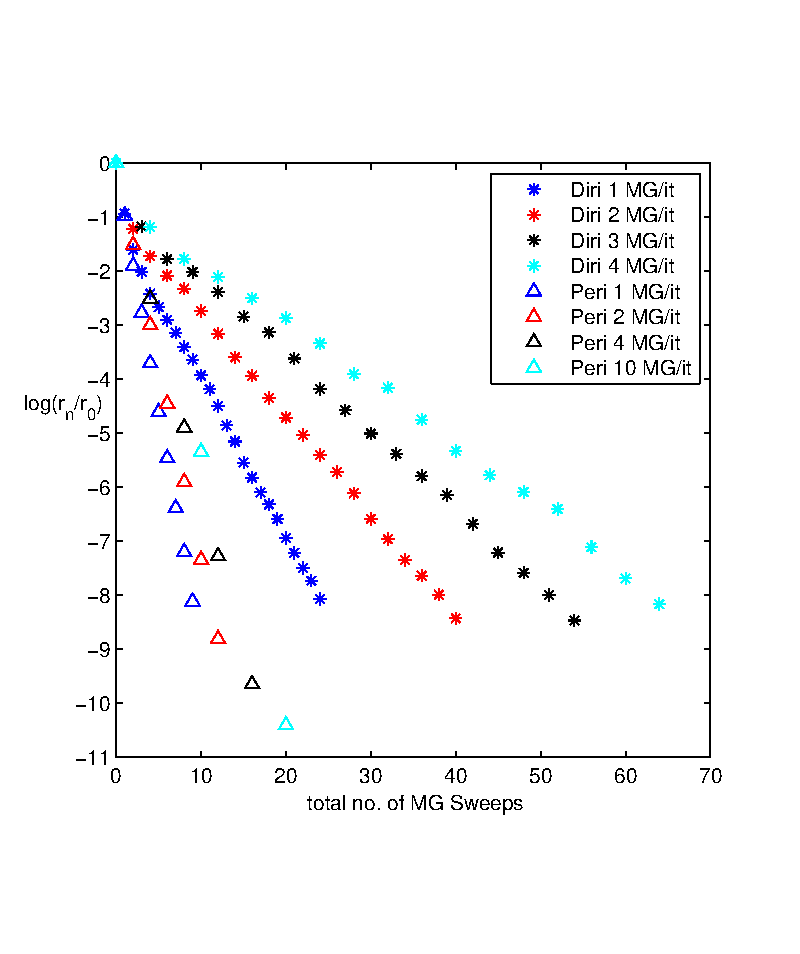
\includegraphics[height=5.6cm]{logRelRes_Vs_diffMGsweeps_Diri_Period_2d}
\hskip .1cm
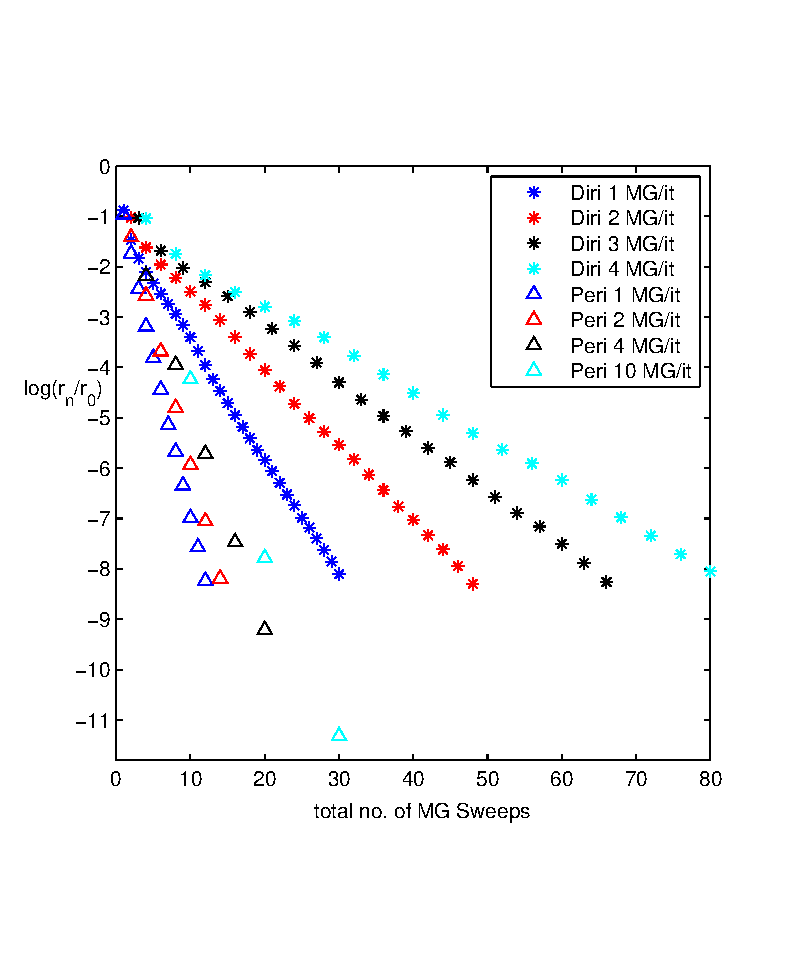
\includegraphics[height=5.6cm]{logRelRes_Vs_diffMGsweeps_Diri_Period_3d}
\vskip .1cm {Figure 1. Log of the norm of the relative residual Vs. the total number of multigrid sweeps using different numbers of MG sweeps per Krylov iteration. 2D plot(left) and 3D plot(right).}
\end{figure}
From the figure, we see that for pure Dirichlet boundary condition, 1 multigrid sweep per iteration gives us the steepest descent of the relative residual. For pure periodic boundary condition, there is little difference.

In the second test, we report the effects of the boundary conditions. The number of multigrid sweep per iteration is 1(which has been proved to be optimal in the first test) but different types of boundary conditions are used to investigate the performance of the solvers. A 3D steady Stokes problem of the size $64\times 64 \times 64$ is used as a benchmark problem. In Figure 2, we report convergence behaviors of the preconditioned FGMRES method using pure Dirichlet BC, $x-$ periodic BC, $xy-$ periodic and pure periodic BC.
\begin{figure}\label{Fig2}
\centering
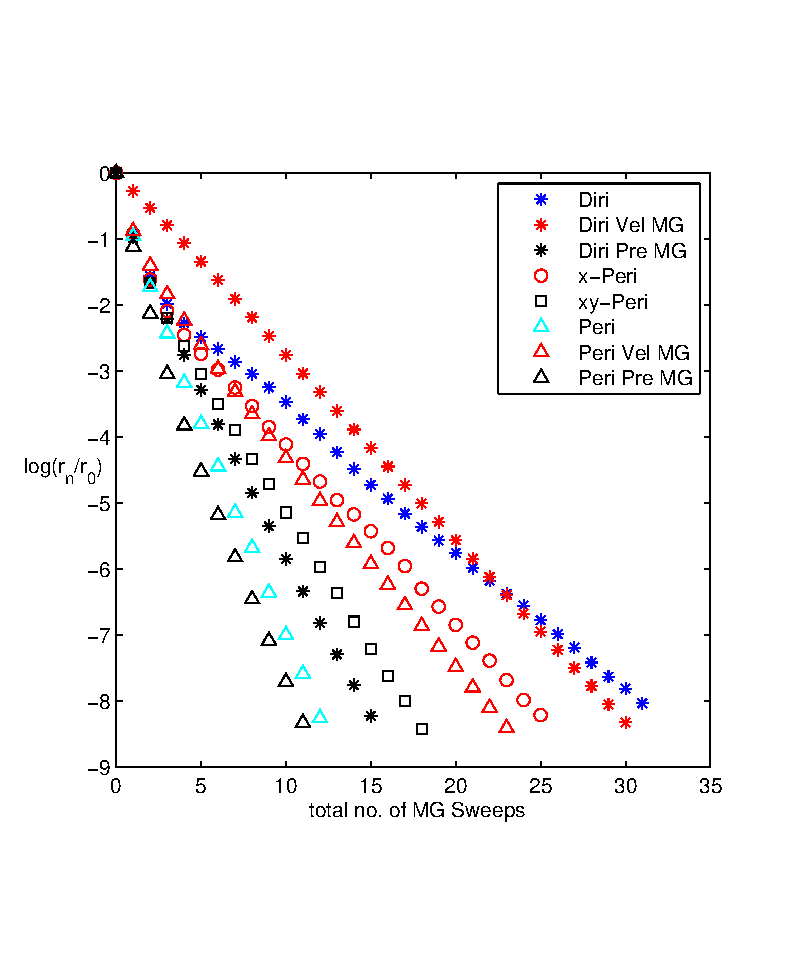
\includegraphics[height=5.6cm]{logRelRes_VsMGsweeps_DiffBC_3d}
\vskip .1cm {Figure 2. Log of the norm of the relative residual Vs. the total number of multigrid sweeps using different boundary conditions.}
\end{figure}
From the figure we see that pure Dirichlet BC needs more total multigrid sweeps to converge to the desired tolerance.

We have done numerical experiments and eigenvalue analysis(see the figures below) to show that there seems to be no significant difference by using left preconditioned GMRES, right precondtioned GMRES or FGMRES (if projection preconditioner is used). Besides, we want to know how to choose restart number so that GMRES (or FGMRES) accelerates the convergence but saving the memory. Therefore, in the third test, we report left preconditioned GMRES with different restart number and compared the results with Richardson iteration (applied to the global preconditioned system). In the test, pure Dirichlet BC is imposed and the problem sizes of the 2D case and 3D case are $256\times256$ and $64\times 64\times 64$ respectively. In Figure 3, the left plot is for the 2D case and the right plot is for the 3D case. We see that restart number can be a small number (10 or 5 even) but can not be too small. Nevertheless, by comparing the results of using GMRES with those using Richardson, we see clearly that GMRES outperforms Richardson.
\begin{figure}\label{Fig3}
\centering
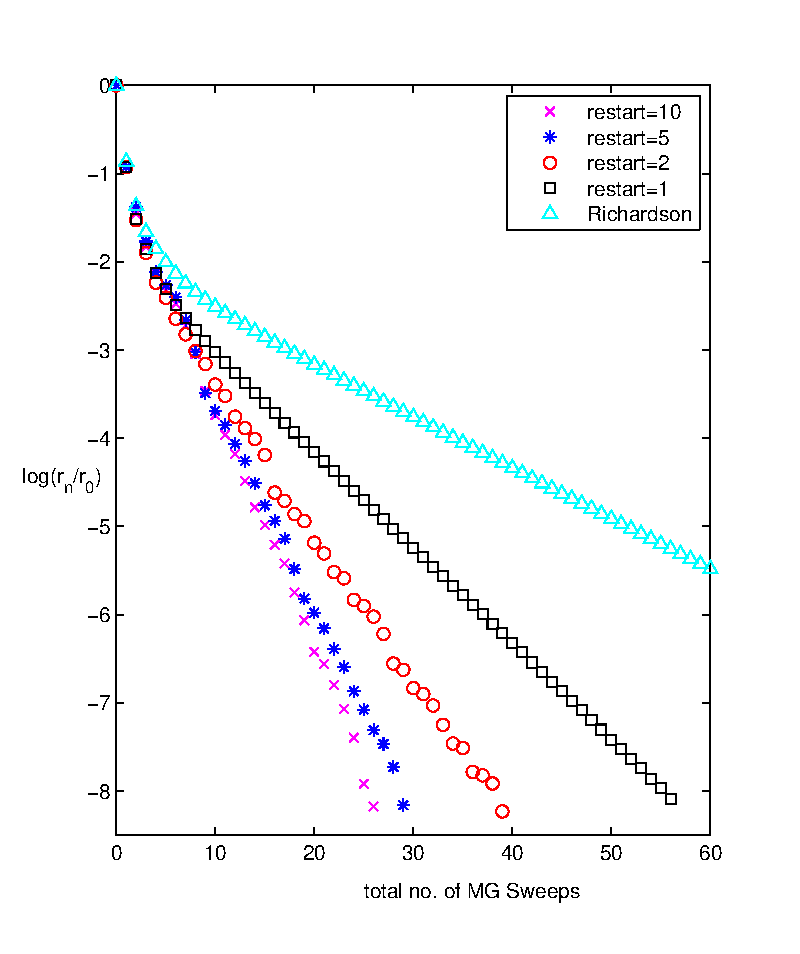
\includegraphics[height=5.6cm]{logRelRes_VsMGsweep_diffRestart_2d}
\hskip .1cm
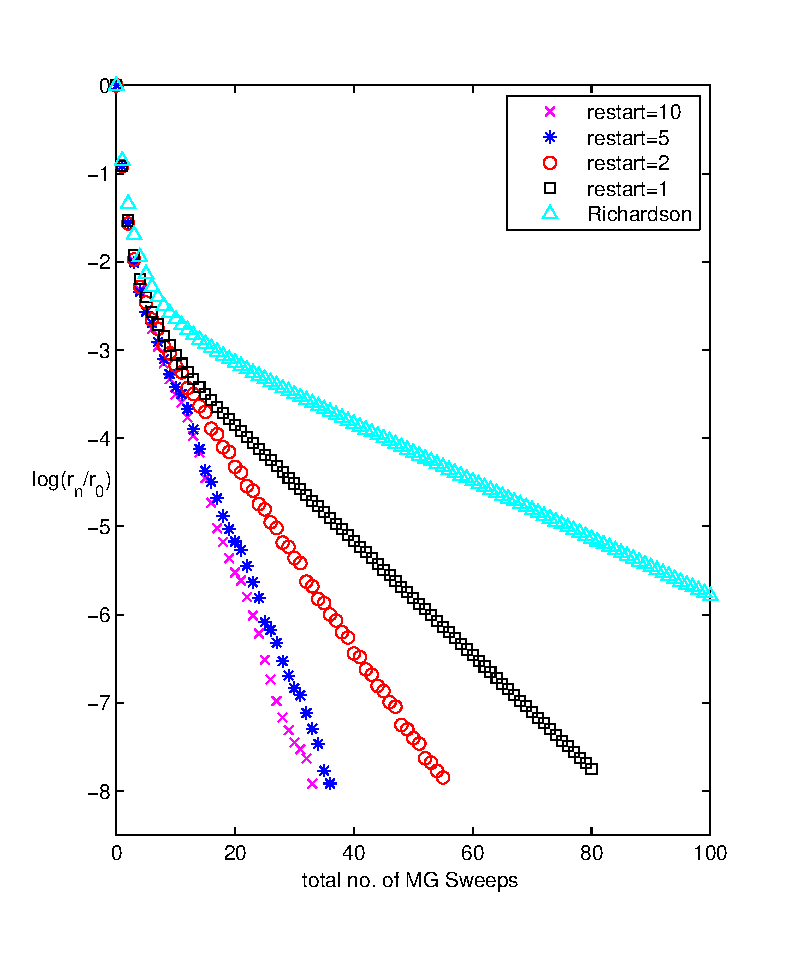
\includegraphics[height=5.6cm]{logRelRes_VsMGsweep_diffRestart_3d}
\vskip .1cm {Figure 3. Log of the norm of the relative residual Vs. the total number of multigrid sweeps for comparing left preconditioned GMRES (with different restart number) and Richardson iteration. 2D plot(left) and 3D plot(right).}
\end{figure}

\subsection{Eigenvalues Plot}
In this subsection, we report some eigenvalue analysis for the projection preconditioner. From (\ref{preconditioned_sys}), we see that the eigenvalue of preconditioned system are either 1 or the eigenvalues of $(\frac{\rho}{\Delta t} {\bf L}_p^{-1} -\mu {\bf I}) {\bf D} {\bf A}^{-1}{\bf G}$. Since numerical experiments indicate that steady state problem needs more iterations, we therefore focus on the eigenvalue analysis of the preconditioned system in stead state case. We assume that the boundary condition is pure Dirichlet and there are $n$ cells in both $x-$ direction and $y-$ direction.

In the following tests, we set $n=2^5$ and use 10 bins to equally distribute the spectrum of the Stokes system and that of the corresponding preconditioned system. In the case of constant viscosity, we are able to prove that there are only $4(n-1)$ eigenvalues not equal to 1. The hist plots of the eigenvalues of Stokes problem (left) and the eigenvalues of preconditioned system are reported in Figure 4. There are around $96\%$ eigenvalues of the preconditioned system are equal to 1.
\begin{figure}\label{Fig4}
\centering
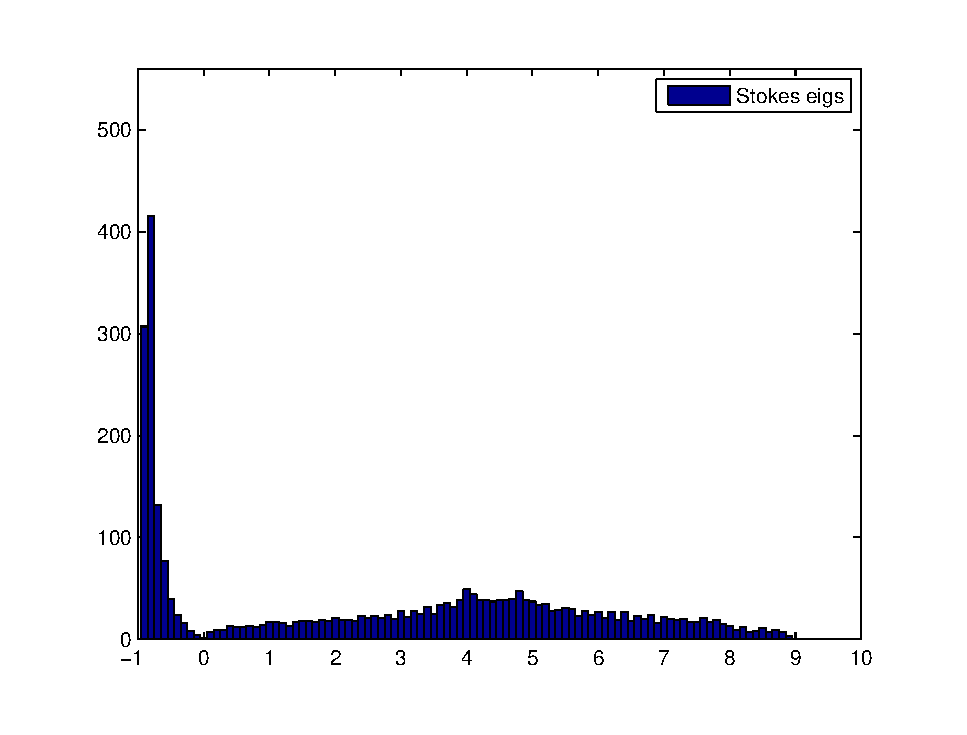
\includegraphics[height=5.6cm]{Stokes_eigs_const_vis}
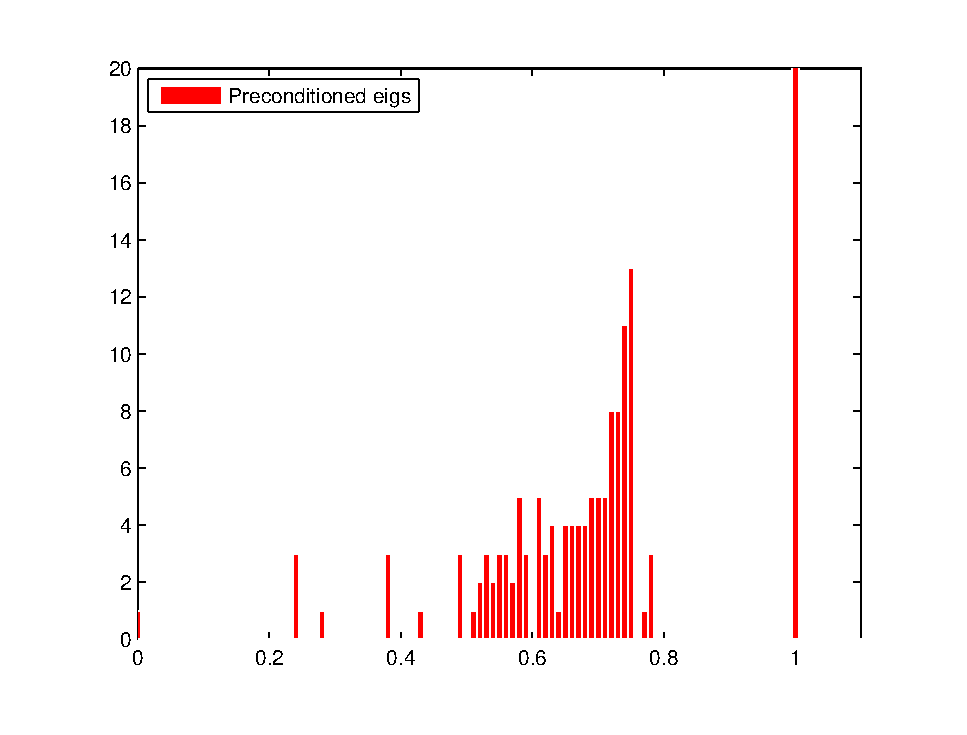
\includegraphics[height=5.6cm]{Preconditioned_eigs_const_vis}
\vskip .1cm {Figure 4. Hist plots of the eigenvalues of the Stokes problem (left) with constant viscosity and the corresponding eigenvalues of the preconditioned system (right). There are around 96\% eigenvalues are equal to 1.}
\end{figure}
For variable viscosity case, we let the viscosity be random, defined by
$$
{\V{\mu}}= {\bf I} + 0.5*{\bf R},
$$
where ${\bf R}$ is a diagonal matrix with the diagonal entries randomly distributed in (0, 1). In Figure 5, we report the hist plots of the spectra of the Stokes problem and the corresponding preconditioned system. We see that the eigenvalues are clustered around 1 even the viscosity is random.
\begin{figure}\label{Fig5}
\centering
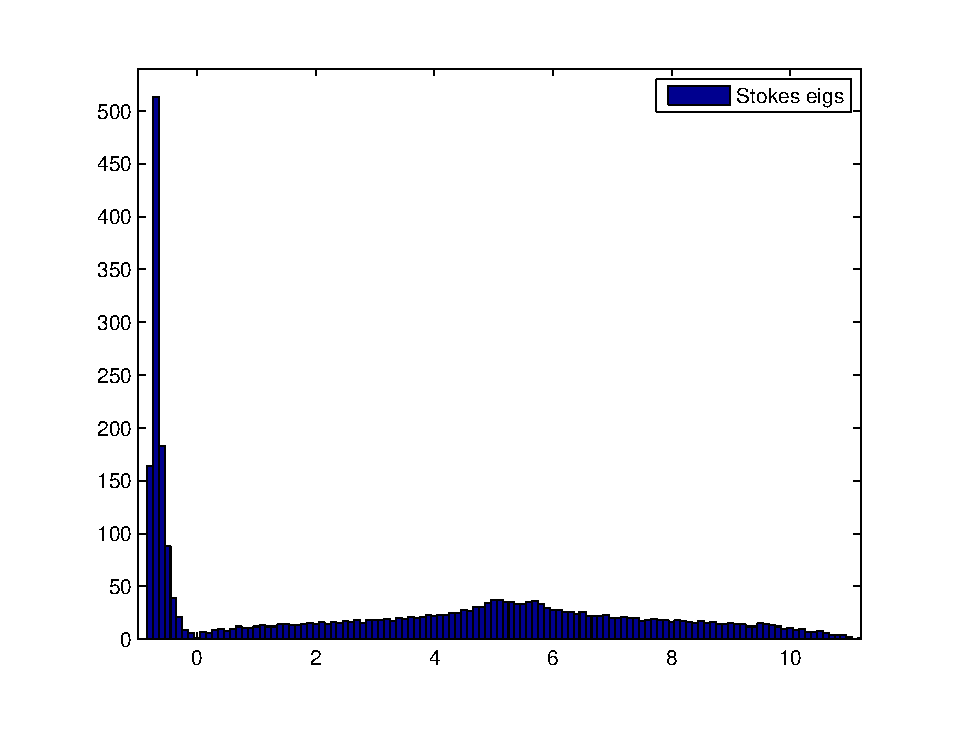
\includegraphics[height=5.5cm]{Stokes_eigs_rand_vis}
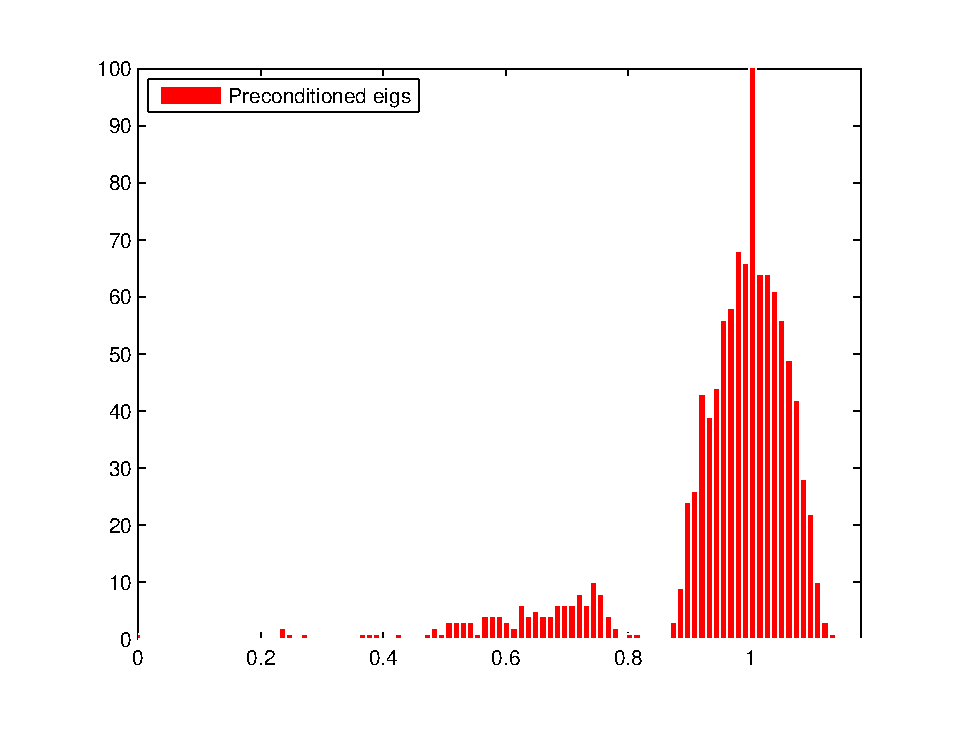
\includegraphics[height=5.5cm]{Preconditioned_eigs_rand_vis}
\vskip .1cm {Figure 5. Hist plots of the eigenvalues of the Stokes problem (left) with constant viscosity and the corresponding eigenvalues of the preconditioned system (right). There are around 82\% eigenvalues are clustered around 1.}
\end{figure}

\section{Experiments for Variable Density Problems.}

In numerical implementation, we avergae $\V{\rho}$ from cell centers to cell faces. Denote ${\bf u}^*=(u, v)^T$, the variable density pressure Poisson solver for solving (\ref{pre_Poisson_eqn}) is as follows.
\begin{eqnarray}\label{dis_Poisson}
-\frac{2}{\Delta x^2}\left(
\frac{\phi_{i+1, j} - \phi_{i,j}}
{{\rho}_{i+1, j} + {\rho}_{i,j}}-
\frac{\phi_{i, j} - \phi_{i-1,j}}
{{\rho}_{i, j} + {\rho}_{i-1, j}}
\right)
 - \frac{2}{\Delta y^2}\left(
\frac{\phi_{i,j+1}- \phi_{i, j}}
{{\rho}_{i,j+1} + {\rho}_{i,j}}-
\frac{\phi_{i,j}- \phi_{i, j-1}}
{{\rho}_{i,j} + {\rho}_{i,j-1}}
\right)\nonumber\\
=
-\frac{1}{\Delta t}\left(
\frac{u^*_{i+\myhalf,j}-u^*_{i-\myhalf,j}}
{\Delta x}
+\frac{v^*_{i, j+\myhalf}-v^*_{i, j-\myhalf}}
{\Delta y} + g_{i,j}\right).
\end{eqnarray}

We test the above 3 preconditioners for variable density Stokes problems. In the following 3 tests, the boundary conditions, the force terms, domain size, mesh size and the time step size are same as those in {\bf Test 1}. The only difference between the following 3 tests and {\bf Test 1} is that density function is defined case by case.

\begin{table}[h]
\begin{center}
\begin{tabular}{|c||ccc|ccc|ccc|}
\hline
BC     &    &1    &  &   & 2    &  &   &4     & \\
\hline
$\mu $   &$N_2$ &$N_3$  &$N_4$  &$N_2$ &$N_3$  &$N_4$    &$N_2$  &$N_3$  &$N_4$ \\
\hline
\hline
$1000$    &18   &15  &22     &12  &10  &15      &5   &4  &3 \\
\hline
$100$     &16   &14  &18     &12  &10  &14      &6   &4  &4 \\
\hline
$10$      &13   &12  &11     &10  &9   &10      &5   &4  &4 \\
\hline
$1$       &10   &9   &7      &8  &8    &6      &4   &3  &3 \\
%\hline
%$\mu =1$ & $7$    &     &9    &9    &6       &8  &8  &6   &    &4   &3  &3 \\
\hline
$0.1$     &7   &6   &4       &6   &5  &4       &4   &3   &3 \\
\hline
$0.01$    &5   &4   &3       &4   &3  &3      &3   &3   &3 \\
\hline
$0$       &2   &2   &2       &2   &2  &2      &2   &1   &1 \\
\hline
\end{tabular}
\vspace{2mm} \caption{Stokes problem with {\bf smoothly varying density}.
}
\end{center}
\end{table}

{\bf Test 2.} The values of $\V{\rho}$ at cell centers are evaluated by using the density function
$$
\rho(x, y) = 1+  r \mbox{cos}\left(\frac{2 \pi x}{L_x}\right)\mbox{sin} \left(\frac{2 \pi y}{L_y}\right),
$$
Here $r=0.5$ is the magnitude of density variations.  If $r$ goes to 0, the problem is reduced to the constant density 1 case. (The smaller $r$ is, the less the number of iterations.) Numerical results are reported in Table 2.

\begin{table}[h]
\begin{center}
\begin{tabular}{|c||ccc|ccc|ccc|}
\hline
 BC         &    &1    &   &    &2    &   &4     &      &\\
\hline
$\mu $     &$N_2$ &$N_3$  &$N_4$  &$N_2$ &$N_3$  &$N_4$   &$N_2$  &$N_3$  &$N_4$ \\
\hline
\hline
$1000$    &17    &15    &21     &13  &11  &19     &7   &4  &4 \\
\hline
$100$     &15    &14    &15     &12  &11  &13     &7   &5  &5 \\
\hline
$10$      &12    &11    &9      &10  &10  &9      &8   &6  &6 \\
\hline
$1$        &9    &9     &6      &8   &8   &6      &8   &6  &6 \\
%\hline
%$\mu =1$ &$7$  &      &13     &13   &11   &   &11    &11    &  &10  &9  &8 \\
%\hline
\hline
$0.1$     &6   &6    &5        &6   &6   &5       &6   &5  &5 \\
\hline
$0.01$    &4   &4    &4        &4   &4   &4       &5   &4  &4 \\
\hline
$0.001$   &4   &3    &3        &4   &3   &3       &4   &3  &3 \\
\hline
$0$       &2    &2   &2        &2   &2   &2       &2   &1  &1 \\
\hline
%\hline
%$\mu=10$    &$6$  &    &13  &13   &10   &  &10  &10   &9    &     &8   &6   &6\\   % larger variations
%\hline
%$\mu=0.1$   &$6$  &    &6   &6    &5    &   &6   &6   &4    &     &5   &4   &4 \\
\end{tabular}
\vspace{2mm} \caption{Stokes problem with {\bf randomly varying density}.
}
\end{center}
\end{table}

{\bf Test 3.} The values of $\V{\rho}$ at cell centers are evaluated by
$$
\V{\rho} = {\bf I}+ r {\bf R},
$$
where $r=0.5$ is used to control the magnitude of the fluctuations and ${\bf R}$ is a diagonal matrix with the diagonal entries (values in $(0, 1)$) generated by the Matlab function: {\it rand}. Numerical results are summarized in Table 3.

\begin{table}[h]
\begin{center}
\begin{tabular}{|c||ccc|ccc|ccc|}
\hline
 BC        &    &1    &      &     &2    &    &      &4     & \\
\hline
$\mu$   &$N_2$ &$N_3$ &$N_4$  &$N_2$ &$N_3$  &$N_4$  &$N_2$  &$N_3$  &$N_4$ \\
\hline
\hline
$1000$   &19   &17   &22     &12  &11  &15      &7  &5  &5 \\
\hline
$100$    &16   &14   &17     &12  &11  &14      &7  &5  &5 \\
\hline
$10$     &13   &12   &10     &10  &10  &10      &7  &5  &5 \\
\hline
$1$       &9    &9   &6      &8   &8   &6       &6  &5  &5 \\
%\hline
%$\mu =1$ & $7$    &     &8    &9   &6     &   &7  &8  &6         &   &6  &5  &5 \\
\hline
$0.1$     &6    &6   &4      &6    &5    &4         &5  &4  &4 \\
\hline
$0.01$    &4    &4   &3      &4    &3    &3         &4  &3  &3 \\
\hline
$0$       &2    &2   &2      &2    &2    &2         &2  &1  &1 \\
\hline
\end{tabular}
\vspace{2mm} \caption{Variable density time dependent problem with {\bf $\mbox{tanh}$ smoothed density}.
}
\end{center}
\end{table}

{\bf Test 4.} The values of $\V{\rho}$ at cell centers are evaluated by using the density function
$$
\rho(x, y) = 2+\mbox{tanh}\left(\frac{d({\bf x}, \Gamma)}{h_y} \right),
$$
where $\Gamma$ represents the middle line (parallel to the $x$-axis) of the domain.
In the test, the density ratio is $1:3$. The density function is smoothed by using $\mbox{tanh}$ function, with the interfacial thickness $h_y$. Numerical results are summarized in Table 4.

{\bf Conclusions.} The performance of ${\bf P}_2$, ${\bf P}_3$ and ${\bf P}_4$ for variable density flow problem are quite good. I had tried larger density fluctuations, the performance of ${\bf P}_2$ is as good as that of ${\bf P}_3$.

\section{Preconditioners for Variable Viscosity Stokes Problems.}

\subsection{Stress Forms of Viscous Term.}
Stokes equations with stress form of the viscous term are as follows.
\begin{equation}\label{Stress_NS}
 \left \{
        \begin{array} {ll}
        \V{\rho} \frac{\partial \mathbf{u}}{\partial t} + \nabla p - \nabla \cdot{\taub} = \mathbf{f}, \\
   \nabla\cdot{\bf u}=-g.
        \end{array}
               \right.
\end{equation}
Here, the stress form of the viscous term is
$\taub = {\V{\mu}} \left[\nabla\ub + (\nabla\ub)^T\right].$
Note that, in two dimensions,
\begin{equation}\label{strain_rate}
\taub =
{\V{\mu}} \left[\begin{array}{cc}
2\frac{\partial u}{\partial x} & \frac{\partial u}{\partial y} +\frac{\partial v}{\partial x}\\
\frac{\partial u}{\partial y}+\frac{\partial v}{\partial x} & 2\frac{\partial v}{\partial y}
\end{array}\right],
\end{equation}
and therefore
\begin{equation}\label{div_stress}
\nabla\cdot\taub
=
\left[\begin{array}{l}
2\frac{\partial}{\partial x}\left({\V{\mu}} \frac{\partial u}{\partial x}\right) + \frac{\partial}{\partial y}\left[{\V{\mu}} \frac{\partial u}{\partial y} + {\V{\mu}} \frac{\partial v}{\partial x}\right]  \\
2\frac{\partial}{\partial y}\left({\V{\mu}} \frac{\partial v}{\partial y}\right) + \frac{\partial}{\partial x}\left[{\V{\mu}} \frac{\partial v}{\partial x} + {\V{\mu}} \frac{\partial u}{\partial y}\right]
\end{array}\right].
\end{equation}

{\bf Numerical Scheme.} In our implementation, we solve the Stokes problem,
\begin{equation}\label{orginal_stress_form}
\left(\begin{array}{ccc}
\frac{{\V{\rho}}}{\Delta t}{\bf I}-2\frac{\partial}{\partial x}({\V{\mu}}\frac{\partial}{\partial x})-\frac{\partial}{\partial y}({\V{\mu}} \frac{\partial}{\partial y})     &  -\frac{\partial}{\partial y}({\V{\mu}} \frac{\partial}{\partial x})  & G_x\\
-\frac{\partial}{\partial x}({\V{\mu}} \frac{\partial}{\partial y})      &  \frac{{\V{\rho}}}{\Delta t}{\bf I}-\frac{\partial}{\partial x}({\V{\mu}} \frac{\partial}{\partial x})-2\frac{\partial}{\partial y}({\V{\mu}} \frac{\partial}{\partial y})  & G_y\\
-D_x    &         -D_y         &     {\bf 0}
\end{array}\right)
\left(\begin{array}{c}
{    u^{(n+1)}}  \\
{    v^{(n+1)}} \\
{    p^{(n+1)}}
\end{array}\right)=
\left(\begin{array}{c}
\frac{{\V{\rho}}}{\Delta t}u^{(n)}+{\bf f}_u^{(n)}  \\
\frac{{\V{\rho}}}{\Delta t}v^{(n)}+{\bf f}_v^{(n)}  \\
{    g^{(n)}}
\end{array}\right).
\end{equation}

The discretization of the viscous terms requires ${\V{\mu}}$ at both cell-centers (refer to (\ref{u_xx})) and nodes (see (\ref{v_x}) for example). The value of ${\V{\mu}}$ at a node is simply the average of the four neighboring cell-centered values. Term by term, the discretization of $\nabla\cdot\taub$ for the $x$-component of momentum is as follows.
\begin{equation}\label{u_xx}
\left[\frac{\partial}{\partial x}\left({\V{\mu}} \frac{\partial u}{\partial x}\right)\right]_{i+\myhalf,j} = \frac{({\V{\mu}} \frac{\partial u}{\partial x})_{i+1,j}-({\V{\mu}} \frac{\partial u}{\partial x})_{i,j}}{\Delta x}
\end{equation}
with
\begin{equation}\label{u_x}
\left({\V{\mu}} \frac{\partial u}{\partial x}\right)_{i,j} = {\mu}_{i,j}\left(\frac{u_{i+\myhalf,j} - u_{i-\myhalf,j}}{\Delta x}\right),
\end{equation}
\begin{equation}\label{u_yy}
\left[\frac{\partial}{\partial y}\left({\V{\mu}} \frac{\partial u}{\partial y}\right)\right]_{i+\myhalf,j} = \frac{({\V{\mu}} \frac{\partial u}{\partial y})_{i+\myhalf,j+\myhalf} - ({\V{\mu}} \frac{\partial u}{\partial y})_{i+\myhalf,j-\myhalf}}{\Delta y},
\end{equation}
with
\begin{equation}\label{u_y}
\left({\V{\mu}} \frac{\partial u}{\partial y}\right)_{i+\myhalf,j+\myhalf} = {{\mu}}_{i+\myhalf,j+\myhalf}\left(\frac{u_{i+\myhalf,j+1} - u_{i+\myhalf,j}}{\Delta y}\right),
\end{equation}
\begin{equation}\label{v_xy}
\left[\frac{\partial}{\partial y}\left({\V{\mu}} \frac{\partial v}{\partial x}\right)\right]_{i+\myhalf,j} = \frac{({\V{\mu}} \frac{\partial v}{\partial x})_{i+\myhalf,j+\myhalf} - ({\V{\mu}} \frac{\partial v}{\partial x})_{i+\myhalf,j-\myhalf}}{\Delta y}
\end{equation}
with
\begin{equation}\label{v_x}
\left({\V{\mu}} \frac{\partial v}{\partial x}\right)_{i+\myhalf,j+\myhalf} = {{\mu}}_{i+\myhalf,j+\myhalf}\left(\frac{v_{i+1,j+\myhalf} - v_{i,j+\myhalf}}{\Delta x}\right).
\end{equation}
Similarly, one can discretize $\left[\frac{\partial}{\partial x}\left({\V{\mu}} \frac{\partial v}{\partial x}\right)\right]_{i,j+\myhalf}$, $\left[\frac{\partial}{\partial y}\left({\V{\mu}} \frac{\partial v}{\partial y}\right)\right]_{i,j+\myhalf}$ and $\left[\frac{\partial}{\partial x}\left({\V{\mu}} \frac{\partial u}{\partial y}\right)\right]_{i,j+\myhalf}$.
%is of the order $\mathcal{O}(h^2)$.

{\bf For stress form of the viscous term, Precondtioners $P_2$ and $P_3$ need to be modified a little bit. "2" rather than "1" is scaled in Schur complement approximation.} More precisely, we use
\begin{equation}\label{P2_variable_den_str}
{\bf P}_2^{-1}=\left(\begin{array}{cc}
{\bf A}^{-1} & {\bf 0} \\
{\bf 0}      & {\bf I}
\end{array}\right)
\left(\begin{array}{cc}
{\bf I}     & -{\bf G} \\
{\bf 0}     &  {\bf I}
\end{array}\right)
\left(\begin{array}{cc}
{\bf I}       & {\bf 0} \\
{\bf 0}       & \frac{1}{\Delta t} {\bf L}_{\V{\rho}}^{-1} - 2{\V{\mu}}.
\end{array}\right)
\end{equation}
\begin{equation}\label{P3_variable_density_str}
{\bf P}_3^{-1}=\left(\begin{array}{cc}
{\bf I} & - {\V{\rho}}^{-1}{\bf G} \\
{\bf 0}      & \frac{1}{\Delta t}{\bf I}- 2{\V{\mu}} {\bf L}_{\V{\rho}}
\end{array}\right)
\left(\begin{array}{cc}
{\bf I}     &  {\bf 0} \\
{\bf 0}     &  -{\bf L}_{\V{\rho}}^{-1}
\end{array}\right)
\left(\begin{array}{cc}
{\bf I}     &  {\bf 0} \\
-{\bf D}     &  -{\bf I}
\end{array}\right)
\left(\begin{array}{cc}
{\bf A}^{-1}       & {\bf 0} \\
{\bf 0}            & {\bf I}
\end{array}\right).
\end{equation}
Fourier analysis shows that for ${\V{\mu}}=const = \mu{\bf I}$, the above forms of ${\bf P}_2$ and ${\bf P}_3$ give an exact preconditioner for periodic boundary case.

{\bf Remarks on the scaling of the variable viscosity in preconditioners.} For the implementation of the variable viscosity in the Laplacian operator in velocity variables, there is no doubt that we need to follow the discretization from (\ref{u_xx}) to (\ref{v_x}). However for pressure variable correction, there are two options. One is (as we wrote in (\ref{P2_variable_den_str}) and (\ref{P3_variable_density_str})) directly reshaping ${\V{\mu}}$ into an $nx*ny \times 1$ vector, then scaled with the the vector $({\bf L}_{\V{\rho}}{\bf p})$ (Here {\bf p} is a vector of the size $nx*ny \times 1$ ). (Aleks' comments: Here ${\V{\mu}}$ is a diagonal matrix of cell-centered viscosities. Therefore, 
the face-centered viscosities are not used in the preconditioner. 

Another way seems to be more physical. Note that in the 4th step of projection method, we do
$$
p^{(n+1)}=\phi -  \Delta t \mu  \left({\bf D} {\V{\rho}}^{-1} {\bf G} \right)\phi.
$$
It should be wrote as
\begin{equation}\label{pressure_correction_var}
p^{(n+1)}=\phi -  \Delta t  {\bf D}\left({{\V{\mu}}\V{\rho}}^{-1} {\bf G} \phi \right).
\end{equation}
in variable viscosity case. Then, the viscosity values at cell faces need to calculated (as we have done from (\ref{u_xx}) to (\ref{v_x})). Correspondingly, the (2,2) block in the last matrix of (\ref{P2_variable_den_str}) should be
$$
\displaystyle \frac{1}{\Delta t} {\bf L}_{\V{\rho}}^{-1} - 2{\V{\mu}}=\left(\frac{1}{\Delta t}{\bf I}  - 2{\bf D}\left({{\V{\mu}}\V{\rho}}^{-1} {\bf G}\right)\right){\bf L}_{\V{\rho}}^{-1}.
$$
and the the (2,2) block in the first matrix of (\ref{P3_variable_density_str}) should be
$$
\displaystyle \frac{1}{\Delta t}{\bf I}- 2{\V{\mu}} {\bf L}_{\V{\rho}}=\left(\frac{1}{\Delta t}{\bf I}- 2{\bf D}\left({{\V{\mu}}\V{\rho}}^{-1} {\bf G}\right)\right).
$$
For $P_4$, we do not have the issue of scaling of the variable viscosity. By far, the following tests on variable viscosity problem is based on the first way of scaling. The second way of scaling has also been implemented. For the benchmark tests reported here, there seems to be no difference by using different type of scaling. My tests show that the first way of scaling gives better results than the second.

{\bf Accuracy test.} In this test, we check the local truncation error of MAC discretization of (\ref{div_stress}).
The viscosity values ${\V{\mu}}$ at cell centers are evaluated by $\mu(x, y)=1+\frac{1}{2}\mbox{cos}(2 \pi x)\mbox{sin}(2\pi y)$. The velocity
$$
u(x, y)=\mbox{sin}(2\pi x)\mbox{sin}(2 \pi y), \quad v(x, y)=\mbox{cos}(2 \pi x)\mbox{cos}(2 \pi y).
$$
Then, we derive the viscous terms,
$$
2\frac{\partial}{\partial x}\left(\mu \frac{\partial u}{\partial x}\right) + \frac{\partial}{\partial y}\left[\mu \frac{\partial u}{\partial y} + \mu \frac{\partial v}{\partial x}\right]=-8 {\pi}^2 \mbox{sin}(2 \pi x) \mbox{sin}(2 \pi y)(\mbox{cos}(2 \pi x) \mbox{sin}(2 \pi y)+1),
$$
$$
2\frac{\partial}{\partial y}\left(\mu \frac{\partial v}{\partial y}\right) + \frac{\partial}{\partial x}\left[\mu \frac{\partial v}{\partial x} + \mu \frac{\partial u}{\partial y}\right]=-8 {\pi}^2 \mbox{cos}(2 \pi x)\mbox{cos}(2 \pi y) (\mbox{cos}(2 \pi x)\mbox{sin}(2 \pi y)+1).
$$
Let the domain be $[0, 1]^2$. Assume the boundary conditions are periodic, we calculate the $L^{\infty}$-norm of errors at $(i+\myhalf, j)$ stencils (for $x-$ component, denoted as $e_x$) and errors at $(i, j+\myhalf)$ stencils (for $y-$ component, denoted as $e_y$).
We get second order convergence:
$$
\begin{array}{ccc}
e_x=   1.9059860759, \quad e_y=1.9059860759, \quad \mbox{mesh level}=4, \\
e_x=   0.4989219718, \quad e_y=0.4989219718, \quad \mbox{mesh level}=5.
\end{array}
$$

{\bf Truncation error and global error.} The local truncation errors are highly dependent on boundary treatment. In the interior of the domain, the above discretization leads to $\mathcal{O}(h^2)$ local truncation error. However, when discretizing $\frac{\partial}{\partial x}\left[\mu (x, y)\frac{\partial v}{\partial x}\right]$ near the west and east boundaries (and $\frac{\partial}{\partial y}\left[\mu (x, y)\frac{\partial u}{\partial y}\right]$ near the south and north boundaries), the local truncation error is no longer 2nd order for Dirichlet BC.

The discretization of $u$ near the south boundary by using the low-order (standard) stencils is as follows.
\begin{equation}\label{u_yy_BD_old}
\left[\frac{\partial}{\partial y}\left(\mu \frac{\partial u}{\partial y}\right)\right]_{i+\myhalf,1} \approx \mu _{i+\myhalf,3/2}\left(\frac{u_{i+\myhalf, 2} - u_{i+\myhalf, 1}}{{\Delta y}^2}\right) - \mu_{i+\myhalf, \myhalf}\left(\frac{2u_{i+\myhalf,1}-2u_{i+\myhalf, \myhalf}}{{\Delta y}^2}  \right).
\end{equation}
Here, $u_{i+\myhalf, \myhalf}$ is the $x$- component of velocity at the south boundary. If we use new stencils, we can achieve higher local truncation error. More clearly, (near the south boundary) we apply
\begin{equation}\label{u_yy_BD_new}
\left[\frac{\partial}{\partial y}\left(\mu \frac{\partial u}{\partial y}\right)\right]_{i+\myhalf,1} \approx \mu _{i+\myhalf,3/2}\left(\frac{u_{i+\myhalf, 2} - u_{i+\myhalf, 1}}{{\Delta y}^2}\right) - \mu_{i+\myhalf, \myhalf}\left(\frac{-u_{i+\myhalf,2} + 9u_{i+\myhalf,1}-8u_{i+\myhalf, \myhalf}}{3{\Delta y}^2} \right).
\end{equation}
Similarly, one can approximate $\frac{\partial}{\partial x}\left[\mu (x, y)\frac{\partial v}{\partial x}\right]$ near the west and east boundaries. Bad aspect of this extrapolation technique is that it derstroies the symmetric property.(elliptic operator is symmetric, but the resulted linear system is nonsymmetric.) % Alternatively, one can use flux BC(if we have) to achieve high order accuracy. %For the above mentioned variable coefficient second order derivatives, we need to use flux boundary to achieve high order %accuracy. One sided difference quotient will not give 2nd order accuracy for variable coefficient 2nd order derivatives.
\begin{table}[h]
\begin{center}
\begin{tabular}{|c|cc|cc|cc|}
\hline
%& level  & error  & global error   \\
level     &  ${\V{\varepsilon}}_L^u$  & ${\V{\varepsilon}}_L^v$  &${\bf e}^u$   &${\bf e}^v$   &${\bf e}_g^u$  &${\bf e}_g^v$   \\
\hline
4  &12.02979571 & 3.67437814   &0.01745095  & 0.01445597  & 0.01678862 &  0.01225490   \\
\hline
5  &10.62538441 & 3.19393928   &0.00446305  & 0.00359900  & 0.00436612 &  0.00306054   \\
\hline
6  &10.36082962 & 3.10894608   &0.00112905  & 0.00090133  & 0.00111731 &  0.00076347    \\
\hline
\end{tabular}
\vspace{2mm} \caption{{\bf Truncation error and global error based on the low-order stencils (\ref{u_yy_BD_old}).}}
\end{center}
\end{table}

\begin{table}[h]
\begin{center}
\begin{tabular}{|c|cc|cc|cc|}
\hline
%& level  & error  & global error   \\
level     &  ${\V{\varepsilon}}_L^u$  & ${\V{\varepsilon}}_L^v$  &${\bf e}^u$   &${\bf e}^v$   &${\bf e}_g^u$  &${\bf e}_g^v$   \\
\hline
4  & 2.79233889 & 2.67023744 & 0.01547084  & 0.011844179 & 0.0117863984 & 0.0091449358  \\
\hline
5  & 0.95295248 & 1.32329852 & 0.00391664  & 0.002990635 & 0.0029767052 & 0.0023042844  \\
\hline
6  & 0.34938889 & 0.64611660 & 0.00098442  & 0.000756801 & 0.0007475086 & 0.0005752454  \\
\hline
\end{tabular}
\vspace{2mm} \caption{{\bf Truncation error and global error based on the higher-order stencils (\ref{u_yy_BD_new}).}}
\end{center}
\end{table}

Here, we present the truncation error and global errors for a variable viscosity problem. Denote the truncation error as ${\V{\varepsilon}}_L=[{\V{\varepsilon}}_L^u ~{\V{\varepsilon}}_L^v]^T$. We define a global error as ${\bf e}=[{\bf e}^u ~{\bf e}^v]^T={\bf A}_0^{-1}[{\V{\varepsilon}}_L^u ~{\V{\varepsilon}}_L^v]^T$. We also define a Stokes global error as ${\bf e}_g={\bf M}_0^{-1}[{\V{\varepsilon}}_L ~{\bf 0}]^{T}=[{\bf e}_g^u ~{\bf e}_g^v]^T$ with ${\bf M}_0$ being the steady state Stokes operator here. We set the domain to be $[0.2, 1.2]^2$, and use
$$
\mu(x,y)=1+\frac{1}{2} \mbox{cos}(2 \pi x) \mbox{sin}(2 \pi y); \quad
{\bf u}(x, y)=\left[ \mbox{sin}(2 \pi x) \mbox{sin} (2 \pi y), \mbox{cos} (2 \pi x)\mbox{cos}(2 \pi y) \right]^{T}
$$
for configurations). Dirichlet boundary conditions are applied in both $x$ and $y$ directions. The results are summarized in Table 5 and Table 6. From the results, we see that, for the old stencil discretization, ${\V{\varepsilon}}_L$ is of order $\mathcal{O}(1)$; for the higher-order stencil discretization, ${\V{\varepsilon}}_L$ is of order  $\mathcal{O}(h)$. However, we observe that ${\bf e}$ and ${\bf e}_g$ are of order $\mathcal{O}(h^2)$ for both.
\begin{table}[h]
\begin{center}
\begin{tabular}{|c|c||ccc|ccc|ccc|}
\hline
$ $   &BC     &     &1   &    &    &2    &     &   &4     & \\
\hline
$\rho$  &$\frac{\Delta t}{h^2}$   &$N_2$ &$N_3$ &$N_4$   &$N_2$ &$N_3$ &$N_4$   &$N_2$ & $N_3$ &$N_4$  \\
\hline
\hline
$100$   &$0.5$   &5  &4  &2     &4  &4  &2     &2   &1  &1 \\
\hline
$10$    &$0.5$   &6  &6  &3     &6  &5  &3     &2   &1  &1\\
\hline
$1$     &$0.5$   &9  &8  &6     &7  &7  &5     &2   &1  &1\\
\hline
$0.1$   &$0.5$   &10 &9  &11    &8  &7  &9     &2   &1  &1\\
\hline
$0.01$  &$0.5$   &12 &11 &16    &9  &9  &12    &2   &1  &1\\
\hline
$0.001$ &$0.5$   &13 &12 &18    &9  &9  &13    &2   &1  &1\\
\hline
$0$     &$0.5$   &15 &14 &20   &11  &10 &15    &2   &1  &1\\
\hline
\end{tabular}
\vspace{2mm} \caption{Stress form of viscous term ({\bf Constant viscosity and constant density}).
}
\end{center}
\end{table}

\subsection{Numerical Experiments.}

{\bf Test 7.} We firstly test {\bf constant density and constant viscosity problems} with stress form of viscosity. Problem settings (such as domain size, mesh size, $\Delta t$) are same as those in Table 1. Numerical results are summarized in Table 7.

{\bf Test 8.} We test a {\bf variable viscosity example with analytic solution}: % (Maple file: new\_model6.mw):
$$
u=\mbox{exp}(-8\pi^2t)\mbox{sin}(2 \pi x)\mbox{sin}(2 \pi y); \quad v=\mbox{exp}(-8\pi^2t)\mbox{cos}(2 \pi x)\mbox{cos}(2 \pi y);
$$
$$
p=\mbox{exp}(-16 \pi^2 t)(\mbox{cos}(4 \pi x)+\mbox{cos}(4 \pi y));
\quad
\mu(x,y)=1+\frac{1}{2} \mbox{cos}(2 \pi x) \mbox{sin}(2 \pi y).
$$
Here, $\mu(x,y)$ is used to evaluate the viscosity at cell centers (we also use analytic function to evaluate the viscosity at cell nodes). The computational domain is $[0, 1]^2$. We let $\Delta t$ ($\Delta t  \propto {h_x^2}$) vary so that the viscous CFL number varies.
Numerical results are summarized in Table 8.
\begin{table}[h]
\begin{center}
\begin{tabular}{|c||ccc|ccc|ccc|}
\hline
BC     &     &1   &    &     &2   &     &   &4     & \\
\hline
$\frac{\Delta t}{h^2}$  &$N_2$ &$N_3$ &$N_4$  &$N_2$ &$N_3$ &$N_4$   &$N_2$ & $N_3$ &$N_4$  \\
\hline
\hline
$0.005$    &5  &4   &2    &5  &4  &2      &4   &3  &2 \\
\hline
$0.05$     &7  &6   &4    &6  &5  &3      &5   &3  &2\\
\hline
$0.5$     &10  &9   &6    &8  &7  &5      &6   &4  &3\\
\hline
  $5$     &13 &12   &10   &11 &10 &9      &8   &5  &4\\
\hline
 $50$     &16 &14   &17   &13 &12 &13    &10   &8  &5\\
\hline
$500$     &21 &16   &19   &16 &13 &14    &12   &9  &5\\
\hline
\end{tabular}
\vspace{2mm} \caption{Stress form of viscous term ({\bf smoothly varied viscosity}).
}
\end{center}
\end{table}


\begin{table}[h]
\begin{center}
\begin{tabular}{|c||ccc|ccc|ccc|}
\hline
BC     &     &1    &    &    &2   &     &   &4     & \\
\hline
$\frac{\Delta t}{h^2}$  &$N_2$ &$N_3$ &$N_4$   &$N_2$ &$N_3$ &$N_4$   &$N_2$ & $N_3$ &$N_4$  \\
\hline
\hline
$0.005$    &5  &5  &3     &5  &5  &3     &7   &4   &2 \\
\hline
$0.05$     &7  &7  &4     &7  &7  &4     &9   &6   &3\\
\hline
$0.5$     &11 &11  &6     &11 &10 &7     &11  &8   &4\\
\hline
$5$       &14 &13  &11    &12 &11 &11    &11  &9   &4\\
\hline
$50$      &16  &15  &18   &13 &12 &16    &11  &9   &4\\   % level 6
\hline
$500$     &17  &16  &21   &13 &13 &16    &12  &8  &4\\
\hline
\end{tabular}
\vspace{2mm} \caption{Stress form of viscous term ({\bf randomly varied viscosity}).
}
\end{center}
\end{table}

{\bf Test 9.} {\bf Randomly varied viscosity flow.} The viscosity is given by
$$
{\V{\mu}}  = {\bf I}+ r {\bf R},
$$
Here $r=0.5$ to control the magnitude of fluctuations. Computational domain: $[0, 1]^2$. We set $\rho=1$ and let $\Delta t$ vary so that the viscous CFL number vary. The numerical results are summarized in Table 9, 10.
%Because of the randomness of viscosity, the number of iterations usually range for $P_2$ and $P_3$, we just choose one of the %number of iterations(for illustration).

In Table 9, we summarize the number of iterations of preconditioners for {\bf random viscosity problem with different magnitudes of variations} by using different CFL numbers. In Table 10, we set $\frac{\Delta t}{h^2}=50$. We summarize the numerical results for the cases that the mesh varying from level 5 to level 7.

\begin{table}[h]
\begin{center}
\begin{tabular}{|c||ccc|ccc|ccc|}
\hline
      BC  &     &1    &    &    &2   &     &   &4     & \\
\hline
 level &$N_2$ &$N_3$ &$N_4$   &$N_2$ &$N_3$ &$N_4$   &$N_2$ & $N_3$ &$N_4$  \\
\hline
\hline
  5   &17  &15 &15    &13  &12 &13     &11   &8   &4\\   % level 5
\hline
  6   &16  &15 &18    &13  &12 &16     &11   &9   &4\\   % level 6
\hline
  7   &16  &16 &20    &13  &12 &18     &12   &9   &4\\   % level 7
\hline
\end{tabular}
\vspace{2mm} \caption{Stress form of viscous term ({\bf randomly varied viscosity with mesh refinement}).
}
\end{center}
\end{table}

%\begin{table}[h]
%\begin{center}
%\begin{tabular}{|c|c|ccc|ccc|ccc|}
%\hline
%    &BC    &     &1    &    &    &2   &   &     &4     & \\
%\hline
%$\frac{\Delta t}{h^2}$ & {\bf r}  &$N_2$ &$N_3$ &$N_4$   &$N_2$ &$N_3$ &$N_4$  &$N_2$ & $N_3$ &$N_4$  \\
%\hline
%0.5  &$0.5$     &11  &11   &6     &11 &10 &7      &11  &8   &4\\
%\hline
%0.5  &$0.1$     &9   &9    &6     &8  &8  &6      &8   &5   &3\\
%\hline
%0.5  &$0.01$    &9   &9    &5     &8  &8  &5      &5   &4   &2 \\
%\hline
%0.5  &$0.001$   &9   &8    &6     &8  &7  &5      &4   &3   &2 \\
%\hline
%\hline
%500  &$0.5$     &17  &16  &21     &13  &13  &16    &12  &8  &4\\
%\hline
%500   &$0.1$    &16  &15  &20     &12  &11  &15    &8   &6  &3\\
%\hline
%500   &$0.01$   &15  &13  &19     &11  &9   &14    &7   &4  &2 \\
%\hline
%500  &$0.001$   &14  &13  &19     &10  &9   &14    &5   &3  &2 \\
%\hline
%\end{tabular}
%\vspace{2mm} \caption{Stress form of viscous term ({\bf randomly varied viscosity with different magnitudes of fluctuations}).
%}
%\end{center}
%\end{table}

{\bf Test 11.} {\bf Jump viscosity with a small fluctuations.} The values of ${\V{\mu}}$ at cell centers are generated by
$$
\mu (x, y) = 2+\mbox{tanh}\left(\frac{d({\bf x}, \Gamma)}{h_y} \right)+  0.01 * \mbox{random number}.
$$
Here $\Gamma$ represents the middle line of the domain along $x-$ direction. Numerical results are summarized in Table 11.
\begin{table}[h]
\begin{center}
\begin{tabular}{|c||ccc|ccc|ccc|}
\hline
BC     &     &1     &      &     &2    &     &    &4     & \\
\hline
$\frac{\Delta t}{h^2}$  &$N_2$ &$N_3$ &$N_4$   &$N_2$ &$N_3$ &$N_4$  &$N_2$ & $N_3$ &$N_4$  \\
\hline
\hline
$0.005$    &5  &5  &3     &5  &5  &2     &7   &4   &2 \\
\hline
$0.05$     &7  &7  &4     &7  &7  &4     &10  &6   &4\\
\hline
$0.5$     &11 &11  &8     &10 &9  &7     &11  &8   &5\\
\hline
$5$       &14 &14 &13    &12 &11  &11    &13  &10  &6\\
\hline
$50$      &17 &17 &20    &14 &12  &16    &14  &10  &7\\
\hline
$500$     &19 &19 &21    &14 &13  &17    &15  &11  &7\\
\hline
\end{tabular}
\vspace{2mm} \caption{Stress form of viscous term ({\bf tanh smoothed viscosity with small fluctuations}). }
\end{center}
\end{table}


\begin{table}[h]
\begin{center}
\begin{tabular}{|c||ccc|ccc|ccc|}
\hline
BC     &     &1   &  &   &2   &    &   &4     & \\
\hline
$\frac{\Delta t}{h^2}$  &$N_2$ &$N_3$ &$N_4$   &$N_2$ &$N_3$ &$N_4$   &$N_2$ & $N_3$ &$N_4$  \\
\hline
\hline
$0.005$   &5   &5   &4      &5  &4  &4      &6   &4  &4 \\
\hline
$0.05$    &6   &6   &5      &6  &6  &5      &8   &6  &5\\
\hline
$0.5$     &9   &9   &6      &9 &10  &6      &10  &8  &6\\
\hline
$5$       &12  &12  &9     &11 &11  &9      &11  &9  &8\\
\hline
$50$      &15  &14 &15     &14 &13 &14      &11  &9  &7\\
\hline
$500$     &17  &16 &21     &14 &13 &17      &12  &8   &6\\
\hline
\end{tabular}
\vspace{2mm} \caption{Stokes problem with stress form of viscous term ({\bf both density and viscosity are random}).}
\end{center}
\end{table}

{\bf Test 12.} {\bf Both density and the viscosity are random.} The density is given by
$$
\V{\rho} = {\bf I}+ r {\bf R}.
$$
and the viscosity is given by
$$
{\V{\mu}} = {\bf I}+ r {\bf R}.
$$
We set $r=0.5$ and let $\Delta t$ vary so that the CFL number varies. Computational domain $[0, 1]^2$. Numerical results are summarized in Table 12.

\subsection{Laplacian Formulation for Variable Viscosity Stokes System.}
From (\ref{div_stress}) and the equation of mass conservation, we can also manipulate the global system first.
We solve an equivalent formulation of Stokes system.
\begin{equation}\label{AD_stress_form}
\left(\begin{array}{ccc}
\frac{{\V{\rho}}}{\Delta t}{\bf I}-\frac{\partial}{\partial x}(\mu \frac{\partial}{\partial x})-\frac{\partial}{\partial y}(\mu \frac{\partial}{\partial y})     &  -\frac{\partial}{\partial y}(\mu \frac{\partial}{\partial x})+\frac{\partial}{\partial x}(\mu \frac{\partial}{\partial y})  & G_x\\
-\frac{\partial}{\partial x}(\mu \frac{\partial}{\partial y})+\frac{\partial}{\partial y}(\mu \frac{\partial}{\partial x})      &  \frac{{\V{\rho}}}{\Delta t}{\bf I}-\frac{\partial}{\partial x}(\mu \frac{\partial}{\partial x})-\frac{\partial}{\partial y}(\mu \frac{\partial}{\partial y})  & G_y\\
-D_x     &         -D_y         &     {\bf 0}
\end{array}\right)
\left(\begin{array}{c}
{    u}  \\
{    v} \\
{    p}
\end{array}\right)=
\left(\begin{array}{c}
{\bf f}_u+\left(\frac{\partial \mu g}{\partial x} \right)  \\
{\bf f}_v+\left(\frac{\partial \mu g}{\partial y} \right)  \\
{    g}
\end{array}\right).
\end{equation}
When the {\bf viscosity is constant}, $\frac{\partial}{\partial y}(\mu \frac{\partial}{\partial x})-\frac{\partial}{\partial x}(\mu \frac{\partial}{\partial y})=\frac{\partial}{\partial x}(\mu \frac{\partial}{\partial y})-\frac{\partial}{\partial y}(\mu \frac{\partial}{\partial x}) = 0$, this form reduces to the Laplacian form for constant viscous term. Therefore, ${\bf P}_2$ and ${\bf P}_3$ do not have factor of two in the Schur complement. On discrete level, backward Euler scheme is applied to the above form and each term is treated similar to that in (\ref{u_x})-(\ref{v_x}) except that
$$
\left[\frac{\partial}{\partial x}\left(\mu \frac{\partial v}{\partial y}\right)\right]_{i+\myhalf,j}=\frac{(\mu \frac{\partial v}{\partial y})_{i+1,j} - (\mu \frac{\partial v}{\partial y})_{i, j}}{\Delta x}
$$
and
$$
\left(\frac{\partial \mu g}{\partial x} \right)_{i+\myhalf, j}=\frac{(\mu g)_{i+1, j}-(\mu g)_{i,j}}{\Delta x}.
$$

{\bf Equivalence of numerical solutions based on different forms of Stokes equations.} For both constant viscosity and variable viscosity cases, we have tested several examples to show that the Laplacian formulation of Stokes equation (\ref{AD_stress_form}) is equivalent to (\ref{orginal_stress_form}) within the solver tolerance.


\begin{table}[h]
\begin{center}
\begin{tabular}{|c||ccc|ccc|ccc|}
\hline
 BC      &    &1     &   &   &2     &    &    &4     & \\
\hline
$\frac{\Delta t}{h^2}$  &$N_2$ &$N_3$  &$N_4$  &$N_2$ &$N_3$  &$N_4$  &$N_2$  &$N_3$  &$N_4$ \\
\hline
\hline
$0.005$    &5    &4   &3     &5  &4  &3     &5    &4   &3 \\
\hline
$0.05$     &7    &6   &4     &6  &5  &3     &5    &3   &3 \\
\hline
$0.5$     &11   &10   &7     &9  &8  &6     &6    &4   &4 \\
\hline
$5$       &15   &14  &12    &12  &11 &10    &8    &6   &5 \\
\hline
$50$      &19   &17  &19    &15  &14 &16   &11    &9   &7 \\
\hline
$500$     &27   &22  &22    &20  &16 &17   &14   &11   &8 \\
\hline
\end{tabular}
\vspace{2mm} \caption{Stokes problem ({\bf Laplacian form of the viscosity}) with {\bf Smoothly varied viscosity}.
}
\end{center}
\end{table}
{\bf Test 13}. We test a {\bf variable viscosity example with analytic solution} as in {\bf Test 8}.% (Maple file: new\_model6.mw):
Computational domain $[0, 1]^2$. We let $\Delta t$ ($\Delta t  \propto {h^2}$) vary so that the viscous CFL number varies.
Numerical results are summarized in Table 13.

{\bf Test 14}. The viscosity is given by
$$
{\V{\mu}}  = {\bf I}+ r {\bf R}.
$$
Computational domain $[0, 1]^2$. We set $\rho=1$, $r=0.5$ and let $\Delta t$ vary so that the CFL number varies. The numerical results are summarized in Table 15.

\begin{table}[h]
\begin{center}
\begin{tabular}{|c|ccc|ccc|ccc|}
\hline
 BC     &     &1  &  &     & 2  &  &   &4    & \\
\hline
$\frac{\Delta t}{h^2}$    &$N_2$ &$N_3$ &$N_4$   &$N_2$ &$N_3$ &$N_4$  &$N_2$ & $N_3$ &$N_4$  \\
\hline
$0.005$    &6  &6  &5     &6  &6  &5      &8   &4  &3 \\
\hline
$0.05$     &7  &8  &5     &7  &8  &5      &10  &6  &5\\
\hline
$0.5$      &13 &13  &7    &11 &12  &7     &14  &10 &6\\
\hline
$5$        &19 &19 &14    &16 &16 &13     &16  &11 &6\\
\hline
$50$       &23 &23 &23    &18 &18 &21     &16  &11 &6\\
\hline
$500$      &26 &26 &26    &19 &19 &23     &16  &11 &6\\
\hline
\end{tabular}
\vspace{2mm} \caption{Stokes problem ({\bf Laplacian form of the viscosity}) with {\bf Random viscosity.}}
\end{center}
\end{table}


{\bf Test 15}. Both density and the viscosity are random. The density is given by
$$
\V{\rho} = {\bf I}+ r {\bf R}
$$
and the viscosity is given by
$$
\V{\mu}  = {\bf I}+ r {\bf R}.
$$
In the tests, $r=0.5$. Computational domain $[0, 1]^2$. Numerical results are summarized in Table 15.


\begin{table}[h]
\begin{center}
\begin{tabular}{|c|ccc|ccc|ccc|}
\hline
   B C     &     &1    &     &     & 2     &     &    &4     & \\
\hline
$\frac{\Delta t}{h^2}$   &$N_2$ &$N_3$ &$N_4$  &$N_2$ &$N_3$ &$N_4$  &$N_2$ & $N_3$ &$N_4$  \\
\hline
$0.005$    &5  &5    &4      &5  &4   &4      &6   &4    &4 \\
\hline
$0.05$     &7  &6    &5      &7  &6   &5      &9   &5    &6\\
\hline
$0.5$     &10  &10   &7     &10 &10   &7     &11   &9    &7\\
\hline
$5$       &15  &15  &10     &13 &13  &10     &13  &11    &7\\
\hline
$50$      &19  &19  &16     &16 &16  &15     &14  &11    &7\\
\hline
$500$     &22  &22  &23     &18 &17  &19     &15  &11    &7\\
\hline
\end{tabular}
\vspace{2mm} \caption{Stokes problem {\bf Laplacian form of the viscosity}. ({\bf both density and viscosity are random}).}
\end{center}
\end{table}


{\bf By comparing Table 8 with Table 13 (Table 12 with Table 15), it seems that there is no signifcant difference for the number of iterations of preconditioners by using different forms of the viscous term.}


%\input{references}
\begin{thebibliography}{00}
\bibitem{BellCollelaGlaz}
J. Bell, P. Colella, and H. Glaz, A second-order projection method for the incompressible Navier-Stokes equations. J. Comput. Phys. 85 (1989), no. 2, pp. 257-283.

\bibitem{Benzi}
M. Benzi, G. Golub and J. Liesen, Numerical solution of saddle point problems, Acta Numerica. 2005

\bibitem{CahouetChabard}
J. Cahouet and J. Chabard, Some fast 3D finite element solvers for the generalized Stokes problem. Internat. J. Numer. Methods Fluids 8 (1988), no. 8, 869-895.

\bibitem{Chorin}
A. Chorin, Numerical solution of the Navier-Stokes equations. Math. Comp. 22 1968 pp. 745-762.

\bibitem{Griffith}
B. Griffith. An accurate and efficient method for the incompressible Navier-Stokes equations using the projection method as a preconditioner. J Comput Phys. 228: 7565-7595 (2009).

\bibitem{MardalWinther2004}
K. A. Mardal and R. Winther, Uniform preconditioners for the time dependent Stokes problem. Numer. Math. 98 (2004), no. 2, pp. 305-327.

\bibitem{MardalWinther2011}
K. A. Mardal, and R. Winther, Preconditioning discretizations of systems of partial differential equations. Numer. Linear Algebra Appl. 18 (2011), no. 1, pp. 1-40.

\bibitem{Murphy1}
M. F. murphy, G. H. Golub, and A. J. Wathen, A note on
preconditioning for indefinite linear systems, SIAM J. Sci. Comput.,
21 (2000), pp. 1969-1972.
\bibitem{Orszag}
S.A. Orszag, M. Isreaeli and M.O. Deville, Boundary conditions for incompressible flows
J. Sci. Comput., 1 (1986), p. 75-111.


\end{thebibliography}
% Set the ending of a LaTeX document



% Set the ending of a LaTeX document
\end{document}
